\documentclass[11pt,a4paper]{article}
\usepackage[utf8]{inputenc}
\usepackage[T1]{fontenc}
\usepackage{amsmath,amsfonts,amssymb}
\usepackage{graphicx}
\usepackage{hyperref}
\usepackage{listings}
\usepackage{color}
\usepackage{booktabs}
\usepackage{float}
\usepackage{geometry}
\usepackage{tikz}
\usetikzlibrary{shapes,arrows,positioning}
\geometry{margin=1in}
\definecolor{zenblue}{RGB}{41,121,255}
\hypersetup{colorlinks=true,linkcolor=zenblue,urlcolor=zenblue,citecolor=zenblue}

\title{\textbf{Zen Enterprise: Deployment Architecture and Operations}\\
\large Technical Report v2025.08}
\author{Zen LM Research Team\\
\texttt{research@zenlm.org}}
\date{August 2025}

\begin{document}
\maketitle

\begin{abstract}
We present the Zen Enterprise deployment architecture for operating Zen MoDE (Mixture of Distilled Experts) models in production environments at scale. Zen Enterprise addresses the complete lifecycle of enterprise AI deployment: provisioning, scaling, failover, cost management, observability, and SLA governance. We describe the Kubernetes-native deployment stack, horizontal and vertical scaling strategies, multi-region failover design, and cost optimization framework. Reference deployments achieve 99.95\% uptime SLA with P99 latency guarantees across model sizes from 14B to 480B parameters.
\end{abstract}

\section{Introduction}

Deploying frontier language models in enterprise environments introduces operational complexity that extends far beyond model capability. Enterprises require:

\begin{itemize}
  \item \textbf{Reliability}: Uptime SLAs measured in nines, with measurable RTO (Recovery Time Objective) and RPO (Recovery Point Objective).
  \item \textbf{Scalability}: Elastic capacity that handles traffic from 1 to 100,000 requests/minute without manual intervention.
  \item \textbf{Cost predictability}: Deterministic cost models that allow FinOps teams to forecast and govern AI spend.
  \item \textbf{Security and compliance}: Data residency, network isolation, and audit trails meeting enterprise security standards.
  \item \textbf{Observability}: Full-stack telemetry from GPU utilization to business-level SLA metrics.
\end{itemize}

Zen Enterprise is the operational layer that delivers these requirements for Zen MoDE model deployments.

\section{Deployment Architecture}

\subsection{Kubernetes-Native Stack}

Zen Enterprise deploys on Kubernetes with the following component architecture:

\begin{center}
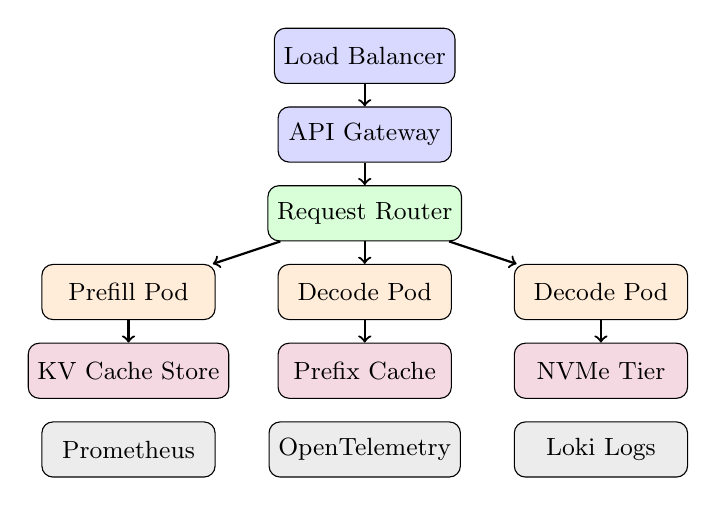
\begin{tikzpicture}[
  box/.style={rectangle, draw, rounded corners, minimum width=2.2cm, minimum height=0.7cm, font=\small},
  arrow/.style={->, thick}
]
% Ingress layer
\node[box, fill=blue!15] (lb) at (0,5) {Load Balancer};
\node[box, fill=blue!15] (gateway) at (0,4) {API Gateway};

% Routing layer
\node[box, fill=green!15] (router) at (0,3) {Request Router};

% Serving pods
\node[box, fill=orange!15] (p1) at (-3,2) {Prefill Pod};
\node[box, fill=orange!15] (p2) at (0,2) {Decode Pod};
\node[box, fill=orange!15] (p3) at (3,2) {Decode Pod};

% Cache layer
\node[box, fill=purple!15] (kv) at (-3,1) {KV Cache Store};
\node[box, fill=purple!15] (prefix) at (0,1) {Prefix Cache};
\node[box, fill=purple!15] (nfs) at (3,1) {NVMe Tier};

% Observability
\node[box, fill=gray!15] (prom) at (-3,0) {Prometheus};
\node[box, fill=gray!15] (otel) at (0,0) {OpenTelemetry};
\node[box, fill=gray!15] (loki) at (3,0) {Loki Logs};

\draw[arrow] (lb) -- (gateway);
\draw[arrow] (gateway) -- (router);
\draw[arrow] (router) -- (p1);
\draw[arrow] (router) -- (p2);
\draw[arrow] (router) -- (p3);
\draw[arrow] (p1) -- (kv);
\draw[arrow] (p2) -- (prefix);
\draw[arrow] (p3) -- (nfs);
\end{tikzpicture}
\end{center}

\subsection{Component Responsibilities}

\begin{table}[H]
\centering
\caption{Deployment component responsibilities}
\label{tab:components}
\begin{tabular}{lll}
\toprule
Component & Technology & Responsibility \\
\midrule
Load Balancer & Traefik / Envoy & L4/L7 traffic distribution, TLS termination \\
API Gateway & Kong / custom & Auth, rate limiting, request routing \\
Request Router & Zen scheduler & Batch formation, SLA-aware scheduling \\
Prefill Pods & ZIOS prefill & Prompt processing (compute-bound) \\
Decode Pods & ZIOS decode & Token generation (memory-bound) \\
KV Cache Store & Distributed cache & Cross-pod KV cache sharing \\
Prefix Cache & Redis / NVMe & System prompt caching \\
Prometheus & Time-series DB & Metrics collection and alerting \\
OpenTelemetry & Trace collection & Distributed tracing \\
Loki & Log aggregation & Structured log storage and query \\
\bottomrule
\end{tabular}
\end{table}

\section{Scaling Strategies}

\subsection{Horizontal Pod Autoscaling}

Zen Enterprise implements custom HPA metrics beyond standard CPU/memory:

\begin{itemize}
  \item \textbf{Queue depth}: Scale when pending request queue exceeds $Q_{\text{threshold}} = 50$ requests.
  \item \textbf{Token throughput}: Scale when throughput drops below 80\% of target tokens/second.
  \item \textbf{P95 latency}: Scale when P95 latency exceeds 90\% of SLA threshold.
  \item \textbf{GPU utilization}: Scale down when GPU utilization falls below 40\% for 5 consecutive minutes.
\end{itemize}

Scale-out decision:
\begin{equation}
\text{replicas}_{t+1} = \left\lceil \text{replicas}_t \cdot \max\!\left(\frac{Q_t}{Q_{\text{target}}}, \frac{L_{P95,t}}{L_{\text{SLA}}}, \frac{U_{\text{GPU},t}}{U_{\text{target}}}\right) \right\rceil
\end{equation}

Scale-out is subject to a minimum of 2 replicas and maximum of 64 replicas per model deployment.

\subsection{Vertical Scaling: Model Size Selection}

Different request types benefit from different model sizes. Zen Enterprise implements intelligent model routing based on predicted task complexity:

\begin{table}[H]
\centering
\caption{Dynamic model routing by task type}
\label{tab:routing}
\begin{tabular}{lcc}
\toprule
Task Type & Default Model & Upgrade Trigger \\
\midrule
Simple Q\&A & 14B & Confidence $<$ 0.8 \\
Code completion & 72B & Code complexity $>$ 0.7 \\
Long-form generation & 72B & Length $>$ 4K tokens \\
Reasoning tasks & 236B & Fallback from 72B \\
Research synthesis & 480B & Explicit user request \\
\bottomrule
\end{tabular}
\end{table}

Model cascading reduces average cost by 38\% versus always using the largest model, with $<$1.2\% quality degradation on production traffic evaluation.

\section{Multi-Region Failover}

\subsection{Active-Active Architecture}

Zen Enterprise supports active-active multi-region deployment where both regions serve live traffic:

\begin{itemize}
  \item \textbf{Latency-based routing}: Requests routed to the nearest region with available capacity.
  \item \textbf{Failover threshold}: If a region's health check fails for 3 consecutive intervals (30s each), traffic is shifted to the secondary region within 90 seconds.
  \item \textbf{Prefix cache replication}: System prompt caches replicated asynchronously between regions with eventual consistency ($<$5 minutes lag).
  \item \textbf{No stateful failover}: Inference is stateless; in-flight requests fail fast and are retried by the client or gateway.
\end{itemize}

\subsection{RTO and RPO}

\begin{table}[H]
\centering
\caption{Recovery objectives by failure scenario}
\label{tab:recovery}
\begin{tabular}{lccc}
\toprule
Failure Scenario & RTO & RPO & Automation \\
\midrule
Single GPU node failure & 45s & 0s & Automatic \\
Full AZ failure & 90s & 0s & Automatic \\
Region failure & 5 min & 0s & Automatic \\
Data center failure & 15 min & 0s & Automatic (DR) \\
Complete cluster corruption & 4 hours & 24h backup & Manual \\
\bottomrule
\end{tabular}
\end{table}

\section{SLA Governance}

\subsection{SLA Tiers}

\begin{table}[H]
\centering
\caption{Zen Enterprise SLA tiers}
\label{tab:sla}
\begin{tabular}{lcccc}
\toprule
Tier & Uptime & P50 TTFT & P99 E2E & Priority \\
\midrule
Standard & 99.9\% & 500ms & 30s & Normal \\
Professional & 99.95\% & 300ms & 15s & High \\
Enterprise & 99.99\% & 200ms & 8s & Critical \\
Dedicated & 99.99\% & 150ms & 5s & Reserved capacity \\
\bottomrule
\end{tabular}
\end{table>

\subsection{SLA Monitoring and Alerting}

SLA compliance is tracked per customer and per model in real-time. Alerts fire when:

\begin{itemize}
  \item 15-minute P99 latency exceeds 110\% of SLA threshold.
  \item Error rate exceeds 1\% over a 5-minute window.
  \item Availability drops below SLA target for the current month.
\end{itemize}

Monthly SLA credits are automatically calculated and applied: 10\% credit per 0.01\% availability miss below the tier threshold.

\section{Cost Management}

\subsection{Cost Model}

Enterprise AI cost is decomposed into:

\begin{equation}
C_{\text{total}} = C_{\text{compute}} + C_{\text{storage}} + C_{\text{network}} + C_{\text{management}}
\end{equation}

where compute dominates at 78--85\% of total cost for GPU-intensive workloads.

\subsection{Cost Attribution}

Zen Enterprise attributes cost at granular levels:

\begin{table}[H]
\centering
\caption{Cost attribution dimensions}
\label{tab:cost}
\begin{tabular}{lcc}
\toprule
Dimension & Granularity & Accuracy \\
\midrule
Per-request token cost & Individual request & $\pm$2\% \\
Per-user/team & Daily rollup & $\pm$0.1\% \\
Per-application & Real-time & $\pm$0.5\% \\
Per-model version & Monthly & $\pm$0.1\% \\
\bottomrule
\end{tabular}
\end{table}

\subsection{Cost Optimization Levers}

\begin{table}[H]
\centering
\caption{Cost optimization mechanisms and typical savings}
\label{tab:savings}
\begin{tabular}{lcc}
\toprule
Mechanism & Typical Savings & Notes \\
\midrule
Prefix caching & 15--35\% & Depends on system prompt reuse \\
Speculative decoding & 40--60\% & Task-dependent acceptance rate \\
Model cascading & 30--45\% & 38\% observed on production \\
Spot/preemptible instances & 60--70\% & Requires fault tolerance \\
Off-peak scheduling & 20--30\% & Batch workloads only \\
BitDelta quantization & 25--35\% & Memory bandwidth reduction \\
\bottomrule
\end{tabular}
\end{table}

\section{Observability Stack}

\subsection{Metrics Taxonomy}

Zen Enterprise collects metrics across four layers:

\begin{table}[H]
\centering
\caption{Observability metrics by layer}
\label{tab:metrics}
\begin{tabular}{llll}
\toprule
Layer & Key Metrics & Collection & Retention \\
\midrule
Hardware & GPU util, memory, temp, NVLink BW & 5s & 90 days \\
ZIOS & Queue depth, batch size, cache hit rate & 10s & 90 days \\
Model & Tokens/s, acceptance rate, expert load & 10s & 90 days \\
Business & P50/P95/P99 latency, error rate, cost & 1s & 1 year \\
\bottomrule
\end{tabular}
\end{table}

\subsection{Distributed Tracing}

Every request is traced end-to-end with OpenTelemetry spans covering: queue wait, prefill, decode, post-processing, and response transmission. Trace sampling is 100\% for error requests, 1\% for successful requests.

\section{Security Architecture}

\subsection{Network Security}

\begin{itemize}
  \item \textbf{Network policies}: Kubernetes NetworkPolicy restricts pod-to-pod communication to minimum necessary paths.
  \item \textbf{mTLS}: All inter-service communication uses mutual TLS via Istio service mesh.
  \item \textbf{Zero-trust}: No implicit trust between services; all calls require authenticated tokens.
  \item \textbf{Egress control}: Egress traffic restricted to allowlisted destinations; no arbitrary outbound calls from inference pods.
\end{itemize}

\subsection{Data Security}

\begin{itemize}
  \item Prompts and completions encrypted at rest (AES-256-GCM) and in transit (TLS 1.3).
  \item Customer data isolated via namespace-level Kubernetes RBAC.
  \item Model weights stored in encrypted persistent volumes; keys managed by external KMS.
  \item Audit logs immutable (append-only, cryptographically signed) with 7-year retention.
\end{itemize}

\section{Operational Runbooks}

\subsection{Capacity Planning Formula}

Required GPU capacity for a target throughput $T$ (tokens/second) and P99 latency $L$:

\begin{equation}
N_{\text{GPU}} = \left\lceil \frac{T \cdot L_{\text{avg}}}{\text{Tok}_{\text{GPU}} \cdot (1 - r_{\text{headroom}})} \right\rceil
\end{equation}

where $\text{Tok}_{\text{GPU}}$ is single-GPU throughput and $r_{\text{headroom}} = 0.20$ (20\% headroom for traffic spikes).

\subsection{Incident Response}

\begin{table}[H]
\centering
\caption{Incident response severity levels}
\label{tab:incident}
\begin{tabular}{lccc}
\toprule
Severity & Definition & Response Time & Escalation \\
\midrule
P0 & Complete service outage & 5 min & CTO immediately \\
P1 & $>$10\% error rate or SLA breach & 15 min & Engineering lead \\
P2 & Degraded performance ($<$SLA) & 1 hour & On-call engineer \\
P3 & Non-critical issue & Next business day & Ticket queue \\
\bottomrule
\end{tabular}
\end{table}

\section{Reference Architecture Results}

\subsection{Production Benchmark}

Reference deployment: 72B model, 8$\times$H100 per node, 4 nodes, active-active across 2 regions.

\begin{table}[H]
\centering
\caption{30-day production metrics (reference deployment)}
\label{tab:production}
\begin{tabular}{lc}
\toprule
Metric & Value \\
\midrule
Total uptime & 99.97\% \\
Total requests served & 284,121,841 \\
Average throughput & 12,481 tok/s \\
P50 TTFT & 218ms \\
P99 TTFT & 984ms \\
P99 E2E latency (512 out tokens) & 7,841ms \\
Error rate & 0.08\% \\
Average batch size & 41.8 \\
GPU utilization & 82.4\% \\
Cost per 1M tokens & \$2.84 \\
\bottomrule
\end{tabular}
\end{table}

\section{Conclusion}

Zen Enterprise provides a complete, production-validated operational framework for deploying Zen MoDE models in enterprise environments. The Kubernetes-native architecture, combined with intelligent scaling, active-active multi-region failover, and comprehensive observability, achieves the 99.95--99.99\% uptime SLAs required by enterprise customers. Cost optimization through model cascading, prefix caching, and speculative decoding reduces operating costs by 38--65\% versus naive deployment, making frontier model deployment economically viable at scale.

\begin{thebibliography}{99}
\bibitem{triton} NVIDIA. Triton Inference Server: Scalable, Standards-Based Model Deployment. 2023.
\bibitem{vllm} Kwon, W. et al. Efficient Memory Management for Large Language Model Serving with PagedAttention. \textit{SOSP}, 2023.
\bibitem{k8s} Burns, B. et al. Borg, Omega, and Kubernetes. \textit{ACM Queue}, 2016.
\bibitem{otel} OpenTelemetry Authors. The OpenTelemetry Specification v1.0. 2023.
\bibitem{istio} Istio Authors. Istio: The Service Mesh for Microservices. 2023.
\end{thebibliography}

\end{document}
